\section{Python}\label{python}
This section will shortly give an overview of the Python programming language version 3.5.1.
This section is based on \citet{python_docs}.

The Python programming language was created by Guido van Rossum in the early 1990s and he is to this day the main author.
As the language has grown there are obviously many more contributors and everyone can contribute as Python is Open Source.

\subsection{some header}
The Python programming language is a dynamic language basically just constructed of lists and dictionaries.
\todo{Noget omkring unicode}

\subsection{Parsing Python}
A Python program uses newlines as delimiters.\footnote{A line can be joined with the next line if it has a ``\texttt{\textbackslash}'' at the end of the line.}
But if an expression is stretched over several lines for instance in parentheses it is still one line but several physical lines.

A comment starts with a ``\texttt{\#}'' symbol.

Indentation is used for grouping statements for instance a body of a function.
The recommended indentation is four spaces.\todo{uvigtigt? ellers skal vi have pep 8 kilde}



Identifiers are unlimited in length and the casing is important.
The following keywords are reserved and cannot be used as identifiers, see \cref{python:keywords_tabular}.
\begin{figure}
  \centering
  \begin{tabular}{l l l l l}
    False & class & finally & is & return \\
None   &    continue &  for     &   lambda  &   try \\
True   &    def     &   from     &  nonlocal &  while \\
and    &    del     &   global   &  not      &  with \\
as     &    elif    &   if        & or       &  yield \\
assert  &   else    &   import   &  pass \\
break   &   except  &   in      &   raise \\
  \end{tabular}
  \caption{Python keywords}
  \label{python:keywords_tabular}
\end{figure}
For a complete list of disallowed identifiers see \citet{python_docs}.

\subsection{Control Structures}\label{python:control_structures}
The python programming language has three control structures, \texttt{if}, \texttt{while} and \texttt{for}.
In the following they are presented as simple examples and a figure showing the possible flow.

\paragraph{\texttt{If}}
The \texttt{if} control structure has several statements:
\begin{enumerate}
\item A simple \texttt{if} statement
\item An \texttt{if-else} statement
\item An \texttt{if-elif-else} statement where the \texttt{elif} statement can be repeated
\end{enumerate}
The \texttt{if} and \texttt{elif} statements contain a condition which is evaluated to either true or false.
If the condition is true the body of the statement is executed if it is false the interpreter will jump to the code after the body.

\begin{figure}
  \centering
  \begin{subfigure}[b]{0.4\textwidth}
    \begin{lstlisting}[style=python, caption={Code example.}, label={python:if:simple:code}]
if True:
    x = 0
    \end{lstlisting}
  \end{subfigure}
  ~ %add desired spacing between images, e. g. ~, \quad, \qquad, \hfill etc. 
  %(or a blank line to force the subfigure onto a new line)
  \begin{subfigure}[b]{0.4\textwidth}
    \centering
    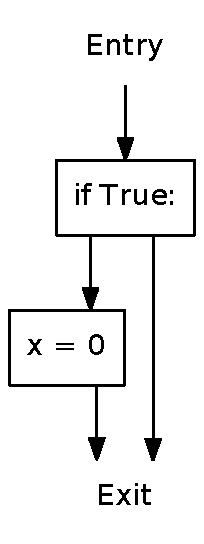
\includegraphics[scale=.5]{./figures/if.pdf}
    \caption{Possible flows.}
    \label{python:if:simple:flow}
  \end{subfigure}
  \caption{A simple \texttt{if} control structure containing one \texttt{if} statement.}
  \label{python:if:simple}
\end{figure}

Taking a look at \cref{python:if:simple} we can see a simple \texttt{if} control structure containing only one \texttt{if} statement.
The code, \cref{python:if:simple:code}, is an \texttt{if} statement with a condition, \texttt{True}.
If the condition holds the body is executed and if not, the program moves on to the next piece of code.
This flow can be seen on \cref{python:if:simple:flow}.


\begin{figure}
  \centering
  \begin{subfigure}[b]{0.4\textwidth}
    \begin{lstlisting}[style=python, caption={Code example.}, label={python:if:else:code}]
if True:
    x = 0
else:
    y = 0
    \end{lstlisting}
  \end{subfigure}
  ~ %add desired spacing between images, e. g. ~, \quad, \qquad, \hfill etc. 
  %(or a blank line to force the subfigure onto a new line)
  \begin{subfigure}[b]{0.4\textwidth}
    \centering
    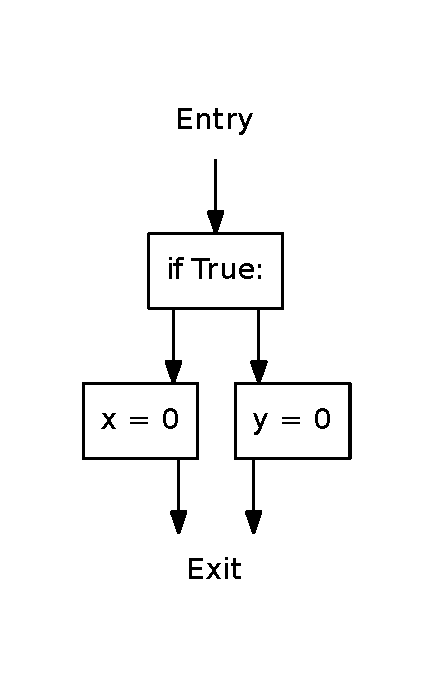
\includegraphics[scale=.5]{./figures/if_else.pdf}
    \caption{Possible flows.}
    \label{python:if:else:flow}
  \end{subfigure}
  \caption{An \texttt{if} control structure containing an \texttt{if} and an \texttt{else} statement.}
  \label{python:if:else}
\end{figure}

A more advanced \texttt{if} control structure can be seen on \cref{python:if:else}.
This example consists of an \texttt{if} statement and an \texttt{else} statement.
The condition of the \texttt{if} statement is evaluated and if it holds the body of the \texttt{if} is executed if not the body of the \texttt{else} is executed.
These possible flows can be seen on \cref{python:if:else:flow}.


\begin{figure}
  \centering
  \begin{subfigure}[b]{0.4\textwidth}
    \begin{lstlisting}[style=python, caption={Code example.}, label={python:if:elif:code}]
if True:
    x = 0
elif False:
    y = 0
else:
    z = 0
    \end{lstlisting}
  \end{subfigure}
  ~ %add desired spacing between images, e. g. ~, \quad, \qquad, \hfill etc. 
  %(or a blank line to force the subfigure onto a new line)
  \begin{subfigure}[b]{0.4\textwidth}
    \centering
    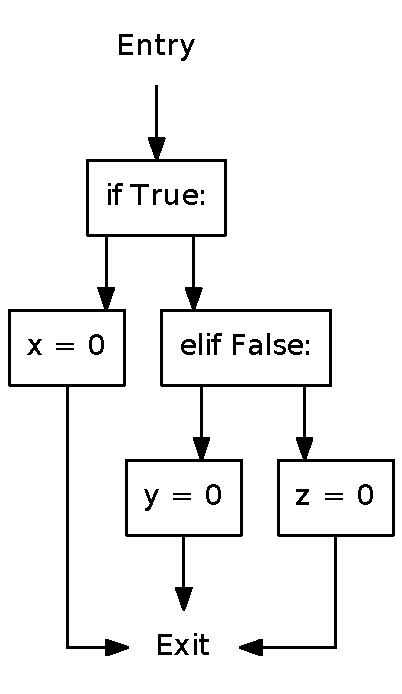
\includegraphics[scale=.5]{./figures/if_else_elif.pdf}
    \caption{Possible flows.}
    \label{python:if:elif:flow}
  \end{subfigure}
  \caption{An \texttt{if} control structure containing an \texttt{if}, an \texttt{elif}, and an \texttt{else} statement.}
  \label{python:if:elif}
\end{figure}


And now the last possible statement in an \texttt{if} control structure the \texttt{if-elif-else} statement.
The \texttt{elif} statement has a condition like the \texttt{if} statement and if it holds its body is executed.
An example can be found on \cref{python:if:elif}.


\paragraph{\texttt{while}}
The \texttt{while} control structure has a condition which evaluates to true or false.
If the condition is true the body is executed and the condition is evaluated again, if it still holds the body is executed again.
This process continuous until the condition is false.
A \texttt{while} control structure can also have an \texttt{else} statement.
The body of the \texttt{else} statement is executed when the condition of the \texttt{while} statement is false.

\begin{figure}
  \centering
  \begin{subfigure}[b]{0.4\textwidth}
    \begin{lstlisting}[style=python, caption={Code example.}, label={python:while:code}]
while x > 0:
    x += 1
    x += 2
print('Done')
    \end{lstlisting}
  \end{subfigure}
  ~ %add desired spacing between images, e. g. ~, \quad, \qquad, \hfill etc. 
  %(or a blank line to force the subfigure onto a new line)
  \begin{subfigure}[b]{0.4\textwidth}
    \centering
    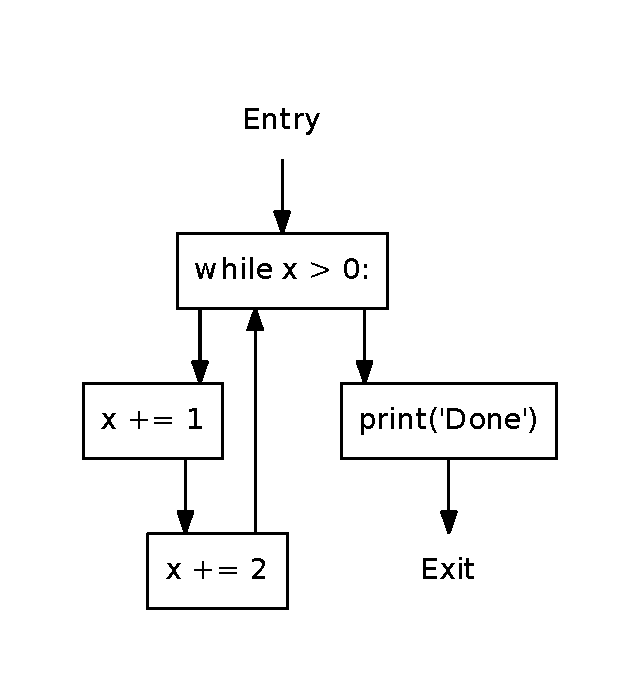
\includegraphics[scale=.5]{./figures/while_no_orelse.pdf}
    \caption{Possible flows.}
    \label{python:while:flow}
  \end{subfigure}
  \caption{A \texttt{while} control structure.}
  \label{python:while}
\end{figure}

For an example we can take a look at \cref{python:while}.
Here we have a simple \texttt{while} control structure with a condition, \texttt{x > 0}.
The possible flows can be seen on \cref{python:while:flow}.
An example with the \texttt{else} statement can be found on \cref{python:while:else}

\begin{figure}
  \centering
  \begin{subfigure}[b]{0.4\textwidth}
    \begin{lstlisting}[style=python, caption={Code example.}, label={python:while:else:code}]
while x < 100:
    x += 1
    x += 2
else:
    x += 3
    x += 4
    \end{lstlisting}
  \end{subfigure}
  ~ %add desired spacing between images, e. g. ~, \quad, \qquad, \hfill etc. 
  %(or a blank line to force the subfigure onto a new line)
  \begin{subfigure}[b]{0.4\textwidth}
    \centering
    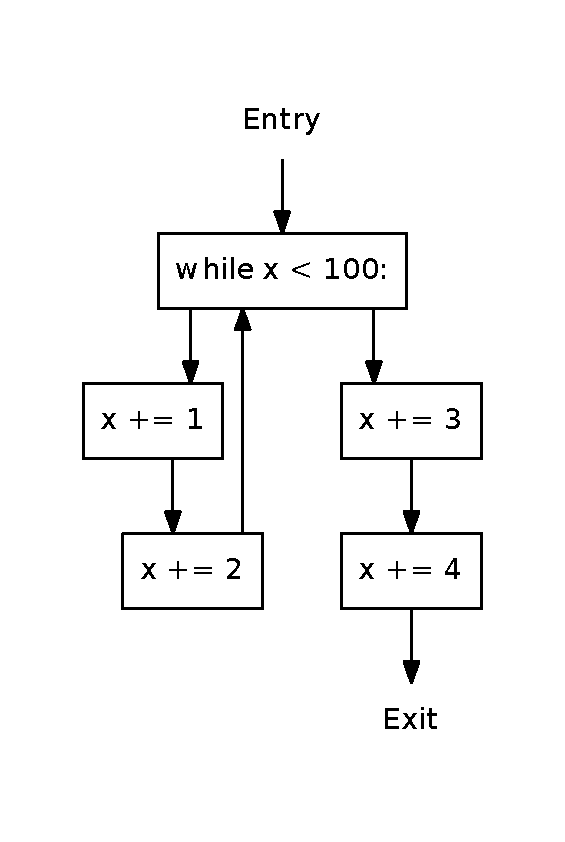
\includegraphics[scale=.5]{./figures/while_else.pdf}
    \caption{Possible flows.}
    \label{python:while:else:flow}
  \end{subfigure}
  \caption{A \texttt{while} control structure.}
  \label{python:while:else}
\end{figure}


\paragraph{\texttt{for}}
The \texttt{for} control structure is used for iterating over an object that is iterable.
This could for instance be a list or a tuple, \cref{}.\todo{ref to list and tuple}
This control structure has an optional \texttt{else} statement, which body is executed when there is nothing to iterate or the \texttt{for} statement is done iterating.
To illustrate the \texttt{for} control structure we provide two examples.
The first example, on \cref{python:for}, shows the most common usage of the \texttt{for} control structure.
Here we iterate over a range, which is described in \cref{}. \todo{ref too built in functions - range}
The second example also has a \texttt{else} statement and can be found on \cref{python:for:else}.


\begin{figure}
  \centering
  \begin{subfigure}[b]{0.4\textwidth}
    \begin{lstlisting}[style=python, caption={Code example.}, label={python:for:code}]
for x in range(3):
    print(x)
    y += 1
x = 3
    \end{lstlisting}
  \end{subfigure}
  ~ %add desired spacing between images, e. g. ~, \quad, \qquad, \hfill etc. 
  %(or a blank line to force the subfigure onto a new line)
  \begin{subfigure}[b]{0.4\textwidth}
    \centering
    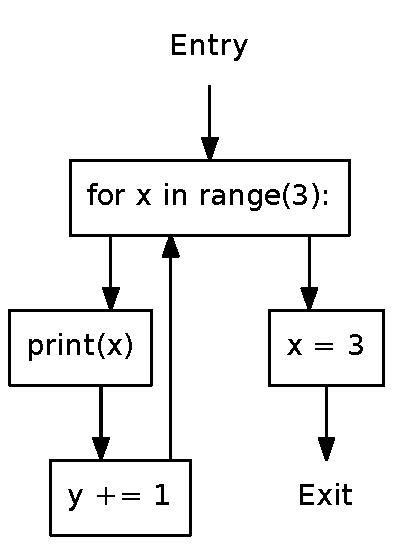
\includegraphics[scale=.5]{./figures/for.pdf}
    \caption{Possible flows.}
    \label{python:for:flow}
  \end{subfigure}
  \caption{A \texttt{for} control structure.}
  \label{python:for}
\end{figure}


\begin{figure}
  \centering
  \begin{subfigure}[b]{0.4\textwidth}
    \begin{lstlisting}[style=python, caption={Code example.}, label={python:for:else:code}]
for x in range(3):
    print(x)
    y += 1
else:
    print(y)
    \end{lstlisting}
  \end{subfigure}
  ~ %add desired spacing between images, e. g. ~, \quad, \qquad, \hfill etc. 
  %(or a blank line to force the subfigure onto a new line)
  \begin{subfigure}[b]{0.4\textwidth}
    \centering
    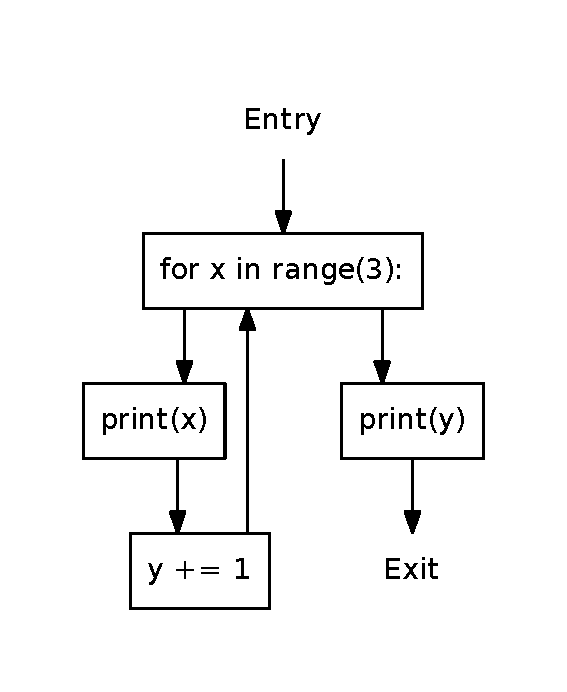
\includegraphics[scale=.5]{./figures/for_complete.pdf}
    \caption{Possible flows.}
    \label{python:for:else:flow}
  \end{subfigure}
  \caption{A \texttt{for} control structure with an \texttt{else} statement.}
  \label{python:for:else}
\end{figure}
